
\documentclass{beamer}
%%%%%%%%%%%%%%%%%%%%%%%%%%%%%%%%%%%%%%%%%%%%%%%%%%%%%%%%%%%%%%%%%%%%%%%%%%%%%%%%%%%%%%%%%%%%%%%%%%%%%%%%%%%%%%%%%%%%%%%%%%%%%%%%%%%%%%%%%%%%%%%%%%%%%%%%%%%%%%%%%%%%%%%%%%%%%%%%%%%%%%%%%%%%%%%%%%%%%%%%%%%%%%%%%%%%%%%%%%%%%%%%%%%%%%%%%%%%%%%%%%%%%%%%%%%%
\usepackage{amsmath}
\usepackage{amssymb}
\usepackage{multirow}
\usepackage{rotating}
\usepackage{verbatim}
\usepackage{multirow}
\usepackage{arydshln}
\usepackage{colortbl}
\usepackage{tabularx}
\usepackage{microtype}
\usepackage{longtable}
\usepackage{dcolumn}
\usepackage{natbib}
\usepackage{tikz}
\usepackage[latin1]{inputenc}
\usepackage{graphicx}
\usepackage{subcaption}
\usepackage{array}
\usepackage{setspace}

\usenavigationsymbolstemplate{}

\usepackage{caption}
\captionsetup{font={footnotesize, singlespacing},skip=-1pt,belowskip=-3pt}

\setcounter{MaxMatrixCols}{10}


\usefonttheme{professionalfonts}
\usefonttheme[]{serif}
\usetheme{Rochester} 
\usecolortheme{beaver}
\usetikzlibrary{shapes,shadows,arrows,shapes.arrows,fadings}
\usefonttheme{professionalfonts}
\institute{Columbia University}
\setstretch{1.1}


\newcounter{myenumi}
\setcounter{myenumi}{0}
\newenvironment{myenumerate}{\begin{enumerate} \setcounter{enumi}{\themyenumi}}{ \setcounter{myenumi}{\theenumi}\end{enumerate}}


\tikzset{My Arrow Style/.style={single arrow, fill=red!50, anchor=base, align=center, text width=1pt, text height=10pt, single arrow head extend=4pt, minimum height=12pt, minimum width=6pt, shape border rotate=0}}
\newcommand*{\tikzarrow}[2][]{\tikz[baseline] \node [My Arrow Style,#1] {#2};}



\begin{document}

\title[SSDS]{Replication of Green \& Vasudevan}
\author{Zenobia Chan, Alicia Cooperman, \& Lauren Young}
\date{October 2015}

\begin{frame}
\titlepage
\end{frame}



\begin{frame}
\frametitle{Overview}

\begin{itemize}
\item Theory
\item Design
\item Replication of main results
\item Robustness to other coding of vote buying
\item Heterogeneous effects
\end{itemize}

\end{frame}


\begin{frame}
\frametitle{Theory}

brief discussion of theory

\end{frame}


\begin{frame}
\frametitle{Design}

Intervention description \\
Does this really test the theory that you've laid out?

\end{frame}



\begin{frame}
\frametitle{Replication process}

Matlab + Stata code \\
No roadmap of order in which code needs to be run to replicate main results 

\end{frame}


\begin{frame}
\frametitle{Main results from the paper}

put up their table - explain the SEs and why they're using SEs from regression and p-values from RI

\end{frame}

\begin{frame}
\frametitle{Correcting standard errors}
Imagine a scenario of 3 clusters with 2 units each.
\begin{columns}[T] % align columns
\begin{column}{.48\textwidth}
\begin{table}[h]
\caption{Constant error variance}
\resizebox{\linewidth} {\height}{%
    \setlength\tabcolsep{2pt}%
\begin{tabular}{ c|c c c c c c|}
 		 &  $e_{11}$ & $e_{12}$ & $e_{21}$ & $e_{22}$ & $e_{31}$ & $e_{32}$\\ \hline
$e_{11}$ & $\sigma^2$ & 0 	   & 0 		  & 0 		 & 0 		& 0 		\\
$e_{12}$ & 0  		 & $\sigma^2$ & 0 		  & 0 		 & 0 		& 0 		\\
$e_{21}$ & 0			 & 0 	   & $\sigma^2$ & 0 		 & 0 		& 0 		\\
$e_{22}$ & 0			 & 0 	   & 0 		  & $\sigma^2$ & 0 		& 0 		\\
$e_{31}$ & 0			 & 0 	   & 0 		  & 0 		 & $\sigma^2$ & 0 		\\
$e_{32}$ & 0			 & 0 	   & 0 		  & 0 		 & 0 		& $\sigma^2$ \\ \hline
\end{tabular}}
\end{table}
\end{column}%
\hfill%
\begin{column}{.48\textwidth}
\begin{table}[h]
\caption{Not-constant error $\Sigma$}
\resizebox{\linewidth} {\height}{%
    \setlength\tabcolsep{2pt}%
\begin{tabular}{ c|c c c c c c|}
 		 &  $e_{11}$ & $e_{12}$ & $e_{21}$ & $e_{22}$ & $e_{31}$ & $e_{32}$\\ \hline
$e_{11}$ & $\sigma_{11}^2$ & 0 	   & 0 		  & 0 		 & 0 		& 0 		\\
$e_{12}$ & 0  		 & $\sigma_{12}^2$ & 0 		  & 0 		 & 0 		& 0 		\\
$e_{21}$ & 0			 & 0 	   & $\sigma_{21}^2$ & 0 		 & 0 		& 0 		\\
$e_{22}$ & 0			 & 0 	   & 0 		  & $\sigma_{22}^2$ & 0 		& 0 		\\
$e_{31}$ & 0			 & 0 	   & 0 		  & 0 		 & $\sigma_{31}^2$ & 0 		\\
$e_{32}$ & 0			 & 0 	   & 0 		  & 0 		 & 0 		& $\sigma_{32}^2$ \\ \hline
\end{tabular}}
\end{table}
\end{column}%
\end{columns}
Var$(\hat{\beta})=(X'X)^{-1}(X' \Sigma X)(X'X)^{-1}$\\
Huber-White ``Robust'' SEs estimate $\hat{\Sigma}$ where $\sigma_i^2$ is $\hat{u}_i^2$ \\
But, still assumes no clustered or spatial correlation
\end{frame}

\begin{frame}
\frametitle{Correcting standard errors}
Imagine a scenario of 3 clusters with 2 units each.\\
Cluster-robust ``block diagonal''
\begin{table}[h]
\caption{Cluster robust}
\begin{tabular}{ c|c c c c c c|}
 		 &  $e_{11}$ 		& $e_{12}$ 		& $e_{21}$ & $e_{22}$ & $e_{31}$ & $e_{32}$\\ \hline
$e_{11}$ & $\sigma_{11}^2$ & $\sigma_{11}\sigma_{12}$ 	   & 0 		  & 0 		 & 0 		& 0 		\\
$e_{12}$ & $\sigma_{12}\sigma_{11}$ & $\sigma_{12}^2$ & 0		  & 0 		 & 0 		& 0 		\\
$e_{21}$ & 0  		 & 0 	   & $\sigma_{21}^2$ & $\sigma_{21}\sigma_{22}$	& 0 		& 0 		\\
$e_{22}$ & 0			 & 0 	   & $\sigma_{22}\sigma_{21}$& $\sigma_{22}^2$ & 0 		& 0 		\\
$e_{31}$ & 0			 & 0 	   & 0 		  & 0 		 & $\sigma_{31}^2$ & $\sigma_{31}\sigma_{32}$\\
$e_{32}$ & 0			 & 0 	   & 0 		  & 0 		 & $\sigma_{32}\sigma_{31}$& $\sigma_{32}^2$ \\ \hline
\end{tabular}
\end{table}
\end{frame}

\begin{frame}
\frametitle{Correcting standard errors}
Imagine a scenario of 3 clusters with 2 units each, \\
but Station 1 covers 11, 12, 21; Station 2 covers cluster 2; Station 3 covers cluster 3.
\begin{table}[h]
\caption{Barrios Dependency Matrix}
\begin{tabular}{ c|c c c c c c|}
 		 &  $e_{11}$ 		& $e_{12}$ 		& $e_{21}$ & $e_{22}$ & $e_{31}$ & $e_{32}$\\ \hline
$e_{11}$ & 1 		& 1	   & 1		  & 0 		 & 0 		& 0 		\\
$e_{12}$ & 1  		& 1 & 1 		  & 0 		 & 0 		& 0 		\\
$e_{21}$ & 1  		& 1	   & 1 & 1 		 & 0 		& 0 		\\
$e_{22}$ & 0			 & 0 	   & 1 & 1 & 0 		& 0 		\\
$e_{31}$ & 0			 & 0 	   & 0 		  & 0 		 & 1 & 1 \\
$e_{32}$ & 0			 & 0 	   & 0 		  & 0 		 & 1 & 1 \\ \hline
\end{tabular}
\end{table}
Multiply this matrix element-by-element with $\hat{u}\hat{u}'$
\end{frame}

\begin{frame}
\frametitle{Correcting standard errors}
Imagine a scenario of 3 clusters with 2 units each, \\
but Station 1 covers 11, 12, 21; Station 2 covers cluster 2; Station 3 covers cluster 3.
\begin{table}[h]
\caption{Barrios $\hat{\Sigma}$}
\begin{tabular}{ c|c c c c c c|}
 		 &  $e_{11}$ 		& $e_{12}$ 		& $e_{21}$ & $e_{22}$ & $e_{31}$ & $e_{32}$\\ \hline
$e_{11}$ & $\sigma_{11}^2$ & $\sigma_{11}\sigma_{12}$ 	   & $\sigma_{11}\sigma_{21}$ 		  & 0 		 & 0 		& 0 		\\
$e_{12}$ & $\sigma_{12}\sigma_{11}$  	 & $\sigma_{12}^2$ & $\sigma_{12}\sigma_{21}$ 		  & 0 		 & 0 		& 0 		\\
$e_{21}$ & $\sigma_{21}\sigma_{11}$  	& $\sigma_{21}\sigma_{12}$ 	   & $\sigma_{21}^2$ & $\sigma_{21}\sigma_{22}$ 		 & 0 		& 0 		\\
$e_{22}$ & 0			 & 0 	   & $\sigma_{22}\sigma_{21}$& $\sigma_{22}^2$ & 0 		& 0 		\\
$e_{31}$ & 0			 & 0 	   & 0 		  & 0 		 & $\sigma_{31}^2$ & $\sigma_{31}\sigma_{32}$\\
$e_{32}$ & 0			 & 0 	   & 0 		  & 0 		 & $\sigma_{32}\sigma_{31}$& $\sigma_{32}^2$ \\ \hline
\end{tabular}
\end{table}
Var$(\hat{\beta})=(X'X)^{-1}(X' \hat{\Sigma} X)(X'X)^{-1}$\\
\end{frame}

\begin{frame}
\frametitle{Main results replicate}

put up our table

\end{frame}



\begin{frame}
\frametitle{What does it mean to be a vote buying party?}

histograms of number of journalists identifying parties as vote buyers

\end{frame}


\begin{frame}
\frametitle{What does it mean to be a vote buying party?}

maps of number of journalists identifying parties as vote buyers

\end{frame}


\begin{frame}
\frametitle{What does it mean to be a vote buying party?}

discussion of dgp for journalists calling a party a vote buyer - innovation of this measure and limitations
discussion of what the right cutpoint is - 100\% of journalists? any?  
 
\end{frame}


\begin{frame}
\frametitle{What does it mean to be a vote buying party?}

regression of 

\end{frame}



\begin{frame}
\frametitle{Are the results sensitive to the defn of vote buying party?}

plot coefficients from range of cutpoints for defn of vote buying party 

\end{frame}


\begin{frame}
\frametitle{Interpretation of the results}

are people just fleeing from the major parties and voting for minor parties?\\
does this change the results? \\
can het effects tell us more about how this works?

\end{frame}


\begin{frame}
\frametitle{Interpretation: Implications for who wins}

In how many PCs do these results change the results?
calc het effects by state and then do projections of which party would have won if the intervention hadn't happened

\end{frame}


\begin{frame}
\frametitle{Heterogeneous effects: Urban}
\begin{columns}[T] % align columns
\begin{column}{.48\textwidth}
\scalebox{.9}{
\vbox{%
\vspace{-10pt}
\begin{table}
Dummy: More than 90\% Rural\\
% latex table generated in R 3.2.2 by xtable 1.7-4 package
% Tue Oct 27 19:21:59 2015
\begin{tabular}{rlll}
  \hline
 & Coef. & SE & p \\ 
  \hline
Treat & -4.68 & 3.6 & 0.1 \\ 
  Rural $>$90 pc & 1.69 & 2.55 & 0.25 \\ 
  Treat:Rural90 & -3.16 & 3.83 & 0.2 \\ 
  R squared & 0.44 &  &  \\ 
   \hline
\end{tabular}

 
\bigskip
Continuous Rural\\
% latex table generated in R 3.2.2 by xtable 1.7-4 package
% Tue Oct 27 17:38:57 2015
\begin{tabular}{rlll}
  \hline
 & ATE & SE & p \\ 
  \hline
Treat & 1.79 & 6.79 & 0.4 \\ 
  Rural pc & -0.01 & 0.05 & 0.45 \\ 
  Treat:Rural pc & -0.1 & 0.06 & 0.06 \\ 
  R squared & 0.44 &  &  \\ 
   \hline
\end{tabular}


\end{table}}}
\end{column}%
\hfill%
\begin{column}{.48\textwidth}
\vspace{-10pt}
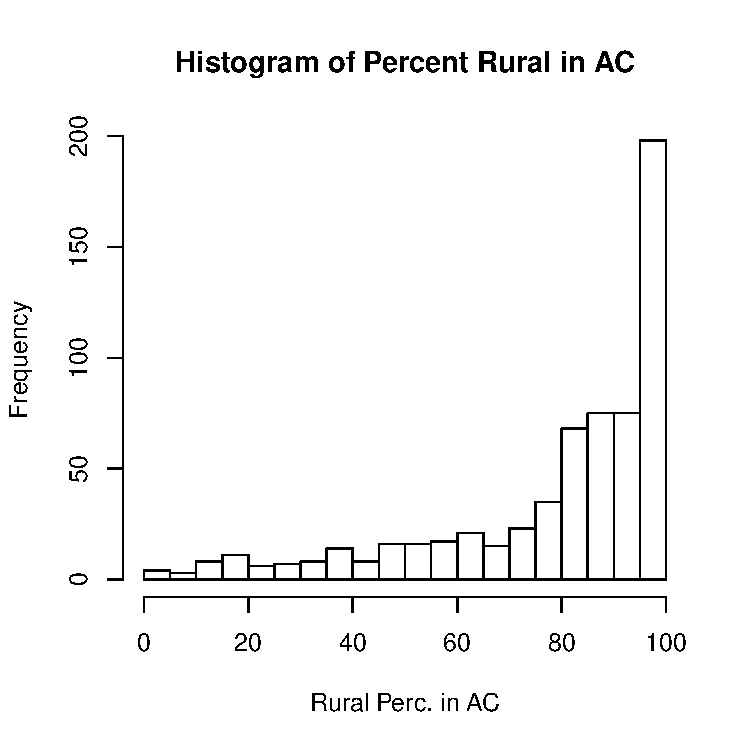
\includegraphics[scale=.45]{../Figures/histrurpc.pdf}
\end{column}%
\end{columns}
\end{frame}

\begin{frame}
\frametitle{Heterogeneous effects: Minority voters}
\begin{columns}[T] % align columns
\begin{column}{.48\textwidth}
\scalebox{.9}{
\vbox{%
\vspace{-10pt}
\begin{table}
Dummy: More than 50\% SC/ST \\
% latex table generated in R 3.2.2 by xtable 1.7-4 package
% Tue Oct 27 19:22:06 2015
\begin{tabular}{rlll}
  \hline
 & Coef. & SE & p \\ 
  \hline
Treat & -6 & 4.4 & 0.09 \\ 
  SC/ST $>$50 pc & -4.88 & 3.66 & 0.09 \\ 
  Treat:SC/ST50 & 1.87 & 5.06 & 0.36 \\ 
  R squared & 0.44 &  &  \\ 
   \hline
\end{tabular}

 
\bigskip
Continuous SC/ST\\
% latex table generated in R 3.2.2 by xtable 1.7-4 package
% Tue Oct 27 17:44:45 2015
\begin{tabular}{rlll}
  \hline
 & ATE & SE & p \\ 
  \hline
Treat & -6.03 & 6.36 & 0.17 \\ 
  ST/SC pc & -0.06 & 0.09 & 0.26 \\ 
  Treat:SC/ST pc & 0.01 & 0.11 & 0.48 \\ 
  R squared & 0.44 &  &  \\ 
   \hline
\end{tabular}


\end{table}}}
\end{column}%
\hfill%
\begin{column}{.48\textwidth}
\vspace{-10pt}
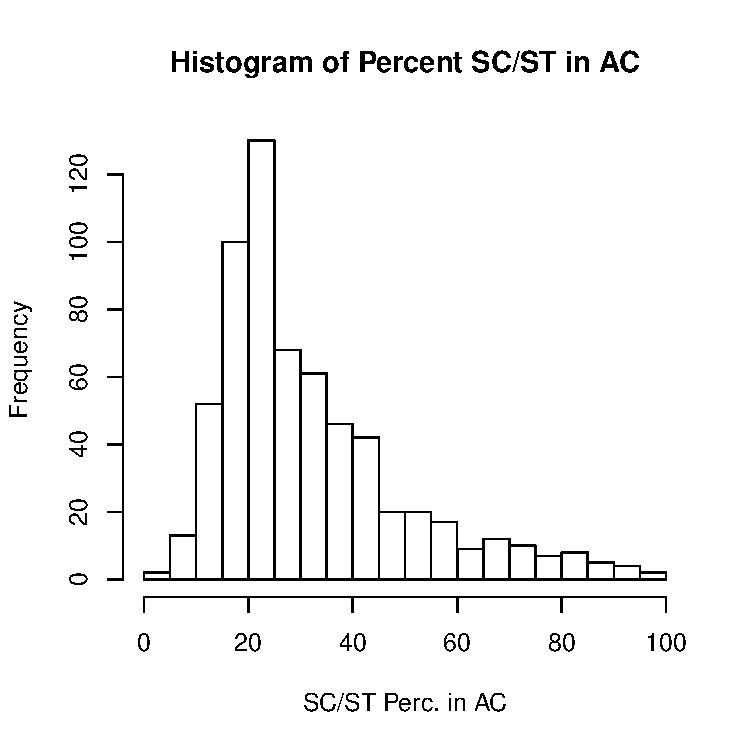
\includegraphics[scale=.45]{../Figures/histscstpc.pdf}
\end{column}%
\end{columns}
\end{frame}



\begin{frame}
\frametitle{Heterogeneous effects: Competitiveness of election}


\end{frame}


\begin{frame}
\frametitle{Heterogeneous effects: State}
\scalebox{.9}{
\vbox{%
\vspace{-10pt}
\begin{table}
\caption{Treatment Status of ACs by State}
% latex table generated in R 3.2.2 by xtable 1.7-4 package
% Tue Oct 27 18:50:48 2015
\begin{tabular}{rrr}
  \hline
 & Control AC & Treated AC \\ 
  \hline
Andhra Pradesh &  82 &  31 \\ 
  Bihar &   0 &  14 \\ 
  Chattisgarh &  15 &  27 \\ 
  Jharkhand &  15 &  17 \\ 
  Karnataka &  50 &  25 \\ 
  Madhya Pradesh &  27 &  18 \\ 
  Maharashtra &  60 &  38 \\ 
  Orissa &  23 &  26 \\ 
  Rajasthan &  42 &  54 \\ 
  Uttar Pradesh &   1 &  63 \\ 
   \hline
\end{tabular}


\end{table}}}
\end{frame}

\begin{frame}
\frametitle{Heterogeneous effects: State}
\begin{columns}[T] % align columns
\begin{column}{.48\textwidth}
\scalebox{.6}{
\vbox{%
\vspace{-10pt}
\begin{table}

% Table created by stargazer v.5.2 by Marek Hlavac, Harvard University. E-mail: hlavac at fas.harvard.edu
% Date and time: Tue, Oct 27, 2015 - 19:03:33
\begin{table}[!htbp] \centering 
  \caption{} 
  \label{} 
\begin{tabular}{@{\extracolsep{5pt}}lc} 
\\[-1.8ex]\hline 
\hline \\[-1.8ex] 
 & \multicolumn{1}{c}{\textit{Dependent variable:}} \\ 
\cline{2-2} 
\\[-1.8ex] & 2014 Vote Share \\ 
\\[-1.8ex] & Vote Buying Parties \\ 
\hline \\[-1.8ex] 
  State Bihar & $-$26.287$^{***}$ (5.571) \\ 
  State Chattisgarh & $-$5.774 (4.893) \\ 
  State Jharkhand & $-$3.946 (4.916) \\ 
  State Karnataka & $-$8.440$^{***}$ (3.115) \\ 
  State Madhya Pradesh & $-$2.123 (3.875) \\ 
  State Maharashtra & $-$4.945$^{*}$ (2.909) \\ 
  State Orissa & $-$4.407 (4.084) \\ 
  State Rajasthan & 1.235 (3.420) \\ 
  State Uttar Pradesh & $-$61.526$^{***}$ (17.276) \\ 
  Vote Share 2009 & 0.588$^{***}$ (0.030) \\ 
  Num Radio 1 & 2.224 (17.458) \\ 
  Num Radio 2 & 1.392 (17.560) \\ 
  Constant & 35.029$^{**}$ (17.569) \\ 
 \hline 
\end{tabular} 
\end{table} 

\end{table}}}
\end{column}%
\hfill%
\begin{column}{.48\textwidth}
\scalebox{.6}{
\vbox{%
\vspace{-10pt}
\begin{table}

% Table created by stargazer v.5.2 by Marek Hlavac, Harvard University. E-mail: hlavac at fas.harvard.edu
% Date and time: Tue, Oct 27, 2015 - 19:03:33
\begin{table}[!htbp] \centering 
  \caption{} 
  \label{} 
\begin{tabular}{@{\extracolsep{5pt}}lc} 
\\[-1.8ex]\hline 
 Treat & 4.353 (3.702) \\ 
  Treat:Bihar &  \\ 
  Treat:Chattisgarh & $-$9.903 (6.618) \\ 
  Treat:Jharkhand & 0.761 (7.062) \\ 
  Treat:Karnataka & $-$3.484 (5.559) \\ 
  Treat:Madhya Pradesh & $-$11.592$^{*}$ (6.357) \\ 
  Treat:Maharashtra & $-$8.632$^{*}$ (5.113) \\ 
  Treat:Orissa & $-$8.085 (6.116) \\ 
  Treat:Rajasthan & $-$14.242$^{***}$ (5.046) \\ 
  Treat:Uttar Pradesh & 43.523$^{**}$ (17.650) \\ 
  Constant & 35.029$^{**}$ (17.569) \\ 
 \hline \\[-1.8ex] 
Observations & 628 \\ 
R$^{2}$ & 0.485 \\ 
Adjusted R$^{2}$ & 0.467 \\ 
Residual Std. Error & 17.111 (df = 606) \\ 
F Statistic & 27.158$^{***}$ (df = 21; 606) \\ 
\hline 
\hline \\[-1.8ex] 
\textit{Note:}  & \multicolumn{1}{r}{$^{*}$p$<$0.1; $^{**}$p$<$0.05; $^{***}$p$<$0.01} \\ 
\end{tabular} 
\end{table} 

\end{table}}}
\end{column}%
\end{columns}
\end{frame}

\begin{frame}
\frametitle{Heterogeneous effects: State}

Map het effects by state

\end{frame}
%
%
%\begin{frame}
%\frametitle{Repression during elections is widespread}
%
%
%\begin{minipage}[t]{0.5\textwidth}
%
%\begin{itemize}
%\item Electoral autocracies and the threat of repression
%\begin{itemize}
%\item 59 of 194 countries are electoral autocracies
%\item Remaining in power often relies on repression
%\item Yet many citizens still choose to mobilize for democracy
%\end{itemize}
%\end{itemize}
%
%\end{minipage}%
%\hspace{0.04\textwidth}%
%\begin{minipage}[t]{0.45\textwidth}
%
%\begin{figure}
%\centering
%\includegraphics[width=.9\textwidth]{../map_neg}
%\end{figure}
%
%\end{minipage}
%
%\vspace{5mm}
%
%\begin{center}
%\textit{How do citizens living in a repressive regime decide to express dissent?}
%\end{center}
%
%%\begin{itemize}
%%\item 46\% of African voters afraid of violence during elections 
%%\item Millions vote for opposition parties
%%\end{itemize}
%
%\end{frame}
%
%%
%%\begin{frame}
%%\frametitle{Citizens weigh costs and benefits of dissent}
%%
%%\begin{itemize}
%%\item Citizens weigh potential costs of dissent against potential benefits \citep{klandermans1984mobilization, kuran1991}. Both are a function of:
%%\begin{itemize}
%%\item The regime's capacity and desire to repress
%%\item The number of other citizens who dissent
%%\end{itemize}
%%\item Repression is a negative potential utility shock \citep{robtor2009, collier2012}
%%%\item The way that expected utility is assessed and processed is not affected by:
%%%\begin{itemize}
%%%\item Uncertain signals
%%%\item High emotions
%%%\end{itemize}
%%\end{itemize}
%%
%%\end{frame}
%
%
%\begin{frame}
%\frametitle{Emotions influence participation in high-risk movements}
%
%\begin{itemize}
%\item Emotions and rationality are substitutes
%\begin{itemize}
%\item Relative deprivation causes anger that creates rebellion \citep{gurr1970}
%\item ``a rush of anger that overwhelms one's deliberative self'' \citep{scott1990domination}
%\end{itemize}
%%\item Case studies argue that emotions matter for participation in
%%\begin{itemize}
%%\item Civil war in El Salvador \citep{wood2003}
%%\item Protest in the civil rights movement \citep{goodwin2009passionate}
%%\end{itemize}
%\item Emotions affect preferences for different strategies
%\begin{itemize}
%\item Expressive utility \citep{kuran1995}
%\item ``Libidinal constitution'' or social ties \citep{goodwin1997libidinal}
%\item Joy of the crowd \citep{lofland1982crowd}
%\item Desire for punishment \citep{halperin2013can}
%\end{itemize}
%\end{itemize}
%
%\end{frame}
%
%
%
%\begin{frame}
%\frametitle{}
%
%
%\begin{figure}
%\centering
%\includegraphics[width=1\textwidth, trim = 100mm 0mm 200mm 0mm, clip = true]{../IMG_4144}
%\end{figure}
%
%
%\end{frame}
%
%\begin{frame}
%\frametitle{Emotions influence behavior through cognition}
%
%\begin{itemize}
%\item Emotions generate quick reactions to threats or opportunities - prepare the brain and body for necessary action \citep{damasio2000feeling}
%%\item The brain sends signals to brain and body to prepare for action
%%\item ``Action tendencies'' work outside of cognitive decisions
%\item Emotions influence cognition through
%\begin{itemize}
%\item Risk perceptions \citep{tversky1983, lernerkeltner2000, lernerkeltner2001}
%\item Risk attitudes
%\item Attention and vigilance 
%\item Cognitive function \citep{eysenck1992anxiety}
%\end{itemize}
%\end{itemize}
%
%\end{frame}
%
%
%
%%
%%\begin{frame}
%%\frametitle{Emotions influence participation in democracy}
%%
%%
%%\begin{itemize}
%%\item Emotions affect participation in democratic politics
%%\begin{itemize}
%%\item Anger increases participation \citep{valentino2009efficacy, valentino2011election}
%%\item Fear has no effect \citep{brader2005}
%%\end{itemize}
%%\item Emotions affect information processing %\citep{marcus2000affective}
%%\begin{itemize}
%%\item Fear increases information seeking \citep{marcus2000affective, valentino2008worried, ryan2012makes} and persuasion \citep{brader2005, brader2006campaigning}, while anger decreases it \citep{mackuen2010civic}
%%\item Anger decreases and fear increases pessimism in perception of foreign policy risks \citep{lerneretal2003}
%%\item Anger decreases depth of processing \citep{lernersmall2008}
%%\end{itemize}
%%\end{itemize}
%%
%%\end{frame}
%
%
%
%\begin{frame}
%\frametitle{Emotions influence participation in democracy}
%
%\begin{table}[ht]
%\centering
%{\scriptsize \begin{tabular}{lp{3.2cm}ccp{3cm}}
%  \hline
% &  Study & \parbox{1cm}{Partici-pation} & \parbox{1cm}{Infor-mation} & DV  \\ 
%  \hline
%\multirow{6}{*}{\rotatebox[origin=c]{90}{\textbf{Anger}}} & \citet{valentino2009efficacy} & $\uparrow$ & & Intention \\
%			& \citet{valentino2011election} & $\uparrow$ &  & Intention, motivation \\
%			& \citet{mackuen2010civic} &  & $\downarrow$  & Information seeking \\
%			& \citet{lerneretal2003} &  & $\downarrow$ & Pessimism \\
%			& \citet{lernersmall2008} &  & $\downarrow$ & Depth of processing \\
%		    & \citet{ryan2012makes} & & $\uparrow$  & Clicking on ad \\
%			\cline{1-5}
%\multirow{6}{*}{\rotatebox[origin=c]{90}{\textbf{Fear}}} & \citet{brader2005} & -  & $\uparrow$ & Intention; Information seeking, persuasion  \\
%		    & \citet{marcus2000affective} & & $\uparrow$ & Information seeking, knowledge \\
%		    & \citet{valentino2008worried} & & $\uparrow$ & Information seeking \\
%		    & \citet{lerneretal2003} &  & $\uparrow$ & Pessimism \\
%   \hline
%\end{tabular}}
%\end{table}
%
%
%\end{frame}
%
%
%
%%
%%\begin{frame}
%%\frametitle{Emotions and other political outcomes}
%%
%%\begin{itemize}
%%\item Democratic politics
%%\begin{itemize}
%%\item Motivation and intention to participate in electoral politics \citep{brader2005, brader2006campaigning, valentino2011election}
%%\item Vigilance and information-seeking \citep{brader2005, brader2006campaigning, ryan2012makes}
%%\end{itemize}
%%\item Contentious politics or violence
%%\begin{itemize}
%%\item Ethnic identification and racism \citep{petersen2012identity, banksvalentino2012, banksbell2013}
%%\item Supporting punitive or aggressive policies \citep{lerneretal2003, halperin2011emotion, halperin2013can}
%%\end{itemize}
%%\end{itemize}
%%
%%\end{frame}
%
%
%
%\begin{frame}
%\frametitle{Theory: Citizens weigh costs and benefits}
%
%%\textcolor{darkred}{Citizens calculate the expected utility of expressing dissent.}
%
%%\vspace{5mm}
%
%\begin{itemize}
%\item Expected costs
%\begin{itemize}
%\item Opportunity cost (time, money)
%\item Risk of repression (probability $\times$ disutility)
%\end{itemize}
%\item Expected benefits
%\begin{itemize}
%\item Self-expression
%\item Potential for change (probability $\times$ utility)
%\end{itemize}
%\item Risk attitudes %= how much citizens would give up to avoid risk
%\end{itemize}
%
%\end{frame}
%
%%
%%\begin{frame}
%%\frametitle{Theory: Decisions to participate in dissent}
%%
%%\begin{figure}
%%\centering
%%\includegraphics[width=.9\textwidth]{../../writeup/decision}
%%\end{figure}
%%
%%\end{frame}
%
%
%
%\begin{frame}
%\frametitle{Theory: Repression events signal risk and induce fear}
%
%Repression events...
%
%\begin{itemize}
%\item Send a credible \textcolor{darkred}{informational signal} of the risk of repression
%\item \textcolor{darkred}{Induce fear} that affects how information is perceived and processed 
%%\begin{itemize}
%%\item Brutality
%%\item Counter-normative
%%\end{itemize}
%\begin{itemize}
%\item Fear increases \textcolor{darkred}{pessimism} about key parameters in the cost of dissent
%\begin{itemize}
%\item The probability of repression
%\item Expectation of whether others will dissent
%\end{itemize}
%\item Fear increases \textcolor{darkred}{risk aversion}
%\end{itemize}
%\end{itemize}
%
%Fear makes repression more effective in reducing dissent
%
%\end{frame}
%
%
%
%
%%\begin{frame}
%%\frametitle{Theory: Assessing the risk of repression}
%%
%%\textcolor{darkred}{Repression events send an \underline{informational signal} about personal risk. }
%%
%%\vspace{5mm}
%%
%%\begin{itemize}
%%\item Regime has an incentive to exaggerate repression risk
%%\item Citizens use past acts of repression as credible signals of own risk
%%\item Still very ambiguous
%%\item Past repression signals higher personal risk when
%%\begin{itemize}
%%\item Closer in time to election
%%\item Victim is more similar to you %(or victim is more visible/high profile)
%%\item Violence is more severe
%%\item Closer in space to you
%%%\item Source is more credible
%%\end{itemize}
%%\end{itemize}
%%
%%\end{frame}
%%
%%
%%
%%\begin{frame}
%%\frametitle{Theory: Assessing the risk of repression}
%%
%%\textcolor{darkred}{Repression events incite \underline{emotions} that change how information is perceived and processed. }
%%
%%\vspace{5mm}
%%
%%\begin{itemize}
%%\item Emotions affect information interpretation and processing
%%\begin{itemize}
%%\item Fear drives pessimism and risk aversion
%%\item Anger increases optimism and risk acceptance
%%\end{itemize}
%%\item Emotions affect key parameters for decisions to dissent
%%\begin{itemize}
%%\item Perceived probability of repression
%%\item Perceived probability that others will dissent
%%\item Risk aversion
%%\end{itemize}
%%\end{itemize}
%%
%%
%%\end{frame}
%
%
%
%
%
%\begin{frame}
%\frametitle{Predictions: The causal effects of fear}
%
%Fear reduces participation in collective dissent. 
%
%\vspace{5mm}
%
%Fear increases the perceived costs of dissent:
%
%\begin{itemize}
%\item Increasing pessimism about others' propensity to dissent
%\item Increasing pessimism about personal risk of repression
%\item Increasing risk aversion
%\end{itemize}
%
%\end{frame}
%
%
%
%\begin{frame}
%\frametitle{Research design: Identifying the effect of emotions}
%
%\begin{itemize}
%\item Goal: Isolate causal effect of fear
%\begin{itemize}
%\item Independent of information about repression
%\item Independent of propensity to feel fear
%\end{itemize}
%\item Design: Experimentally induce fear
%\begin{itemize}
%\item Use directed reflection task from psychology experiments
%\item Induce fear in two contexts
%\begin{itemize}
%\item General fear - cleanest test of the effect of emotions
%\item Political fear - closest to real phenomenon
%\end{itemize}
%\end{itemize}
%\end{itemize}
%
%\end{frame}
%
%
%
%\begin{frame}
%\frametitle{Measuring risky political behavior}
%
%\begin{itemize}
%\item Goals
%\begin{itemize}
%\item Safely measure propensity to take risky action
%\item Measure perceived probabilities with partially innumerate population
%%\item Measure perceived risks independent of selection into risk-taking 
%\end{itemize}
%\item Design
%\begin{itemize}
%\item Measure propensity to take political action in two ways
%\begin{itemize}
%\item Hypothetical: self-reported propensity to take six risky actions
%\item Behavioral: choosing a wristband with a pro-democracy slogan
%\end{itemize}
%\item Measure risk aversion using series of 50-50 lotteries with real payouts
%\item Measure perceived risks 
%\begin{itemize}
%\item on a five-point scales in local language
%\item conditional on a specific action (going to an opposition rally)
%\end{itemize}
%\end{itemize}
%\end{itemize}
%
%\end{frame}
%
%
%
%
%\begin{frame}
%\frametitle{Research design: Measuring perceived risk of repression}
%
%If you went to a rally for an opposition party, how likely is it that you would be...
%
%\begin{itemize}
%\item Threatened
%\item Beaten
%\item Have property destroyed
%\item Abducted
%\item (or a family member) Sexually abused
%\item Killed
%\end{itemize}
%
%Now? Around the next election? 
%
%\end{frame}
%
%
%
%
%%
%%
%%\begin{frame}
%%\frametitle{Empirical strategy: Do emotions affect collective action decisions?}
%%
%%\textbf{Design implementation:} Two lab-in-the-field experiments with 1,200 Zimbabwean opposition supporters
%%
%%\begin{itemize}
%%\item Induce emotions using techniques from psychology
%%\item Measure perceived risk
%%\begin{itemize}
%%\item Five-point scale in vernacular language
%%\item 12-question indices - 6 risks over 2 periods
%%\item In specific situations (how likely is X if you do Y vs. how likely is X given your strategic behavior)
%%\end{itemize}
%%\item Measure risk attitudes with lotteries with real payouts 
%%\item Two measures of propensity to act 
%%\begin{itemize}
%%\item Self-reported index of 12 hypothetical measures
%%\item Behavioral measure based on choosing a political wristband
%%\end{itemize}
%%%\item Double-blind
%%\end{itemize}
%%
%%\end{frame}
%%
%%
%%\begin{frame}
%%
%%\begin{itemize}
%%\item Control for selection into repression risk
%%\item Measurement
%%\begin{itemize}
%%\item Measure perceptions of probabilistic outcomes
%%\item Measure real propensity to take risky behavior safely
%%\end{itemize}
%%\end{itemize}
%%
%%\end{frame}
%%
%
%
%\begin{frame}
%\frametitle{Study context: Repressive electoral autocracy}
%
%\begin{minipage}[t]{0.6\textwidth}
%\begin{itemize}
%\item Electoral autocracy
%\begin{itemize}
%%\item Regularly holds elections that only ruling party can win
%\item Ruling party: liberation movement, took power 1980
%\item Opposition party: MDC, grew out of trade union in 1999
%\end{itemize}
%\item Widespread repression  
%\begin{itemize}
%\item Atrocities in minority region in 1980s
%\item Loss of ruling party popularity 2000
%\item Election violence peaked in 2008%: 180 killed, 9,000 tortured or assaulted, and 28,000 displaced \citep{amnesty2008}
%\end{itemize}
%\item Fieldwork context
%\begin{itemize}
%\item Dominant ruling party
%\item Very low violence against opposition
%%\begin{itemize}
%%\item Swept 2013 election 
%%\item Ran uncontested in 22 by-elections in 2014-2015
%%\end{itemize}
%%\item Factionalization of major parties
%%\item Economy in decline
%\end{itemize}
%\end{itemize}
%\end{minipage}%
%\hspace{0.05\textwidth}%
%\begin{minipage}[t]{0.34\textwidth}
%
%\begin{figure}
%%\includegraphics[width=1\textwidth, trim = 7cm 0mm 0mm 0mm, clip = true]{../zanurally}
%%\includegraphics[width=1\textwidth, trim = 7cm 0mm 0mm 0mm, clip = true]{../../../proposals/zanu_mdc}
%\includegraphics[width=1\textwidth, trim = 1.09cm 0mm 10mm 0mm, clip = true]{../../writeup/militia_zanupf}
%\end{figure}
%
%\end{minipage}
%
%\end{frame}
%
%
%
%\begin{frame}
%\frametitle{Recruiting pro-opposition subjects}
%
%\begin{minipage}[t]{0.45\textwidth}
%\begin{itemize}
%%\item Only opposition supporters
%\item Areas affected by repression
%\item Recruited through established local networks 
%%\item Worked to correct bias towards activists
%\item 1,200 subjects over two experiments
%\end{itemize}	
%\end{minipage}%
%\hspace{0.05\textwidth}%
%\begin{minipage}[t]{0.49\textwidth}
%
%\begin{figure}
%\includegraphics[width=1\textwidth]{../../analysis/graphs/map_sample_all}
%\end{figure}
%
%\end{minipage}
%
%
%\end{frame}
%
%
%
%
%\begin{frame}
%\frametitle{Subjects' have high exposure to and risk of violence}
%
%{\small
%\centering
%\begin{minipage}[t]{0.48\textwidth}
%
%\textbf{Past political violence}
%
%\begin{table}[ht]
%\centering
%\begin{tabular}{lc}
%  \hline
% & Percent  \\ 
%  \hline
%  Threat & 83\% \\ 
%   Discrimination & 63\% \\ 
%  Harm & 38\% \\ 
%  Property & 38\% \\ 
%  Torture & 32\% \\ 
%  Arrest & 17\% \\ 
%  Abduction & 14\% \\ 
%  Sexual & 3\% \\ 
%  Murder & 2\% \\ 
%   \hline
%\end{tabular}
%\end{table}
%
%\end{minipage}%
%\hspace{0.02\textwidth} %
%\begin{minipage}[t]{0.48\textwidth}
%
%\textbf{Perceived risk}
%
%\begin{table}[ht]
%\centering
%\begin{tabular}{lcc}
%  \hline
%  & \multicolumn{2}{c}{\parbox{30mm}{\centering Percent ``Very Likely'' or ``Sure''} }\\
%  \cline{2-3}
% & Current & Election \\ 
%  \hline
%Threat & 25\% & 73\% \\ 
%  Assault & 21\% & 71\% \\ 
%  Abduction & 20\% & 63\% \\ 
%  Property & 20\% & 67\% \\ 
%  Sexual & 19\% & 56\% \\ 
%  Murder & 18\% & 59\% \\ 
%   \hline
%\end{tabular}
%\end{table}
%
%\vspace{4mm}
%
%%{\scriptsize Average risk perception is between ``a little bit'' and ``somewhat'' likely in non-election period, ``very'' likely in election period (except sexual violence).}
%
%\end{minipage}
%}
%
%\end{frame}
%
%
%
%
%
%
%\begin{frame}
%\frametitle{Treatment: Emotion induction}
%
%\begin{itemize}
%\item Psychologists use many ways to induce emotions: videos, music, scenarios, environments, reflection
%\item Reflection task
%\begin{itemize}
%\item Strong enough to show up in brain scans and heart rate
%\item Best way to induce a specific emotion 
%%\item Widely used in political psychology
%\end{itemize}
%\item Implementation
%\begin{itemize}
%\item Usually written, in this case verbal
%\item Enumerators probed until the emotion was induced
%\item 10\% recorded
%\end{itemize}
%\item Blocked on surveyor, gender, and day
%\end{itemize}
%
%\end{frame}
%
%
%\begin{frame}
%\frametitle{Treatment: Emotion induction}
%
%{\scriptsize
%\centering
%\begin{minipage}[t]{0.3\textwidth}
%\textbf{Fear - General}
%
%What are the 2-3 things that make you most \textcolor{darkred}{afraid}? Please tell me in 2-3 sentences about each thing that makes you afraid. You might be afraid of \textcolor{darkred}{witchcraft, being alone on a dark street, being in a traffic accident, or dangerous animals like snakes or lions}.
%
%\end{minipage} %
%\hspace{0.02\textwidth} %
%\begin{minipage}[t]{0.3\textwidth}
%\textbf{Fear - Political}
%
%What are the 2-3 things that make you most \textcolor{darkred}{afraid about politics and elections}? Please tell me in 2-3 sentences about each thing that makes you afraid about politics and elections. You might be afraid of the \textcolor{darkred}{ZANU-PF militia, being abducted, losing your home, or being raped}.
%
%\end{minipage} %
%\hspace{0.02\textwidth} %
%\begin{minipage}[t]{0.3\textwidth}
%\textbf{Control}
%
%What are the 2-3 activities that you do to \textcolor{darkred}{relax}? Please tell me 2-3 sentences about each thing that you like to do. You might feel relaxed when you are \textcolor{darkred}{watching tv, attending soccer matches, reading newspapers and magazines, fishing}.
%
%\end{minipage}
%}
%
%\end{frame}
%
%
%\begin{frame}
%\frametitle{Treatment: Emotion induction}
%
%{\scriptsize
%\centering
%\begin{minipage}[t]{0.3\textwidth}
%\textbf{Fear - General}
%
%Now we'd like you to describe in more detail the one situation that makes you most \textcolor{darkred}{afraid}. This could be something you are presently experiencing or something from the past. Please tell me as if you're trying to make me \textcolor{darkred}{afraid} as well. What is it like to be in this situation? Why is it so \textcolor{darkred}{scary}? \textbf{(X2)}
%\end{minipage} %
%\hspace{0.02\textwidth} %
%\begin{minipage}[t]{0.3\textwidth}
%\textbf{Fear - Political}
%
%Now we'd like you to describe in more detail the one situation that makes you most \textcolor{darkred}{afraid about politics and elections}. This could be something you are presently experiencing or something from the past. Please tell me as if you're trying to make me \textcolor{darkred}{afraid} as well. What is it like to be in this situation? Why is it so \textcolor{darkred}{scary}? \textbf{(X2)}
%\end{minipage} %
%\hspace{0.02\textwidth} %
%\begin{minipage}[t]{0.3\textwidth}
%\textbf{Control}
%
%Now we'd like you to describe in more detail the way you most like to \textcolor{darkred}{relax}. Begin by telling me a description of your favorite \textcolor{darkred}{relaxing activity}. Please tell me as if you're trying to make me \textcolor{darkred}{relaxed} as well. What is it like to be in this situation? Why is it so \textcolor{darkred}{relaxing}? \textbf{(X2)}
%\end{minipage}
%}
%
%\end{frame}
%
%
%
%
%\begin{frame}
%\frametitle{The fear treatments induce large amounts of fear}
%
%\begin{figure}
%\includegraphics[width=.6\textwidth]{../../analysis/graphs/round2/manip_check}
%\end{figure}
%
%\end{frame}
%
%
%
%%\begin{frame}
%%\frametitle{Manipulation checks}
%%
%%\centering
%%{\scriptsize
%%\centering
%%\begin{minipage}[t]{0.3\textwidth}
%%\textbf{Fear - General}
%%
%%\begin{itemize}
%%\item Traffic accidents - 20\%
%%\item Witchcraft - 10\%
%%\item Darkness - 7.5\%
%%\item Violence - 7.5\%
%%\end{itemize}
%%
%%\end{minipage} %
%%\hspace{0.02\textwidth} %
%%\begin{minipage}[t]{0.3\textwidth}
%%\textbf{Fear - Political}
%%
%%\begin{itemize}
%%\item Political violence - 100\%
%%\end{itemize}
%%
%%\end{minipage} %
%%\hspace{0.02\textwidth} %
%%\begin{minipage}[t]{0.3\textwidth}
%%\textbf{Control}
%%
%%\begin{itemize}
%%\item Having money - 45\%
%%\item Peace - 13\%
%%\item Family - 8\%
%%\item Happy marriage - 7\%
%%\end{itemize}
%%
%%\end{minipage}
%%}
%%
%%\vspace{10mm}
%%
%%{\scriptsize Data from Experiment 1}
%%
%%%XX replace with pie charts XX
%%
%%\end{frame}
%
%
%
%\begin{frame}
%\frametitle{Predictions: The causal effects of fear on dissent}
%
%\textcolor{darkred}{Fear reduces participation in collective dissent.}
%
%\vspace{5mm}
%
%Fear increases the perceived costs of dissent:
%
%\begin{itemize}
%\item Increasing pessimism about others' propensity to dissent
%\item Increasing pessimism about personal risk of repression
%\item Increasing risk aversion
%\end{itemize}
%
%\end{frame}
%
%
%
%
%
%\begin{frame}
%\frametitle{Fear reduces dissent}
%
%\begin{figure}
%\includegraphics[width=.7\textwidth]{../../analysis/graphs/round2/density_act}
%\end{figure}
%
%\end{frame}
%
%
%
%
%
%%\begin{itemize}
%%\item Effects are substantively large
%%\begin{itemize}
%%\item Fear causes a 14-25\% reduction in the behavioral measure of dissent
%%\item 
%%\end{itemize}
%%\end{itemize}
%
%
%
%%
%%
%%\begin{frame}
%%\frametitle{Fear decreases propensity to take pro-democracy action}
%%
%%\begin{figure}
%%\includegraphics[width=.5\textwidth]{../../analysis/graphs/round2/coefs_act_ind}
%%\end{figure}
%%
%%\end{frame}
%%
%
%
%\begin{frame}
%\frametitle{Reductions in dissent are substantively important}
%
%\begin{table}[ht]
%\centering
%\begin{tabular}{lccc}
%  \hline
%  & \multicolumn{3}{c}{\parbox{6cm}{\centering Percent ``Very likely'' or ``Sure'' during election period}} \\
%  \cline{2-4}
% & Control & General  & Political \\[-1ex] 
% & & Fear & Fear \\
%  \hline
%%  \textbf{Wristband$^*$} & 81\% & 71\% & 63\% \\
%Shirt & 49\% & 25\% & 24\% \\ 
%  Joke & 28\% & 8\% & 7\% \\ 
%  Rally & 50\% & 36\% & 33\% \\ 
%  Reveal & 39\% & 15\% & 21\% \\ 
%  Refuse & 39\% & 16\% & 16\% \\ 
%  Testify & 31\% & 13\% & 11\% \\ 
%   \hline
%\end{tabular}
%\end{table}
%
%%\footnotesize{$^*$Wristband is a binary behavioral measure of taking the political wristband.}
%
%\end{frame}
%
%
%
%
%
%\begin{frame}
%\frametitle{Fear decreases behavioral propensity to dissent}
%
%\begin{figure}
%\includegraphics[width=.7\textwidth]{../../analysis/graphs/round2/band_means}
%\end{figure}
%
%\end{frame}
%
%
%
%
%
%%\begin{frame}
%%\frametitle{Implications for autocrats and activists}
%%
%%
%%\begin{itemize}
%%\item Strategies of pro-democracy mobilization
%%\begin{itemize}
%%%\item Reduce perceptions of risks %- even if the threat remains constant
%%\item Reduce susceptibility to fear
%%\begin{itemize}
%%\item Increase perceptions of personal efficacy
%%\item Increase ability to manage fear 
%%\end{itemize}
%%\end{itemize}
%%\item The strategic use of violence
%%\begin{itemize}
%%\item Brutal, counter-normative forms of violence are more effective
%%\item Violence must be regularly practiced
%%\item Target repression on citizens susceptible to fear 
%%\begin{itemize}
%%\item Low perceptions of personal efficacy %makes citizens more likely to feel fear
%%\end{itemize}
%%\end{itemize}
%%\end{itemize}
%%
%%
%%\end{frame}
%%
%
%
%
%
%\begin{frame}
%\frametitle{Predictions: The causal effects of fear on cognition}
%
%Fear reduces participation in collective dissent.
%
%\vspace{5mm}
%
%Fear increases the perceived costs of dissent:
%
%\begin{itemize}
%\item \textcolor{darkred}{Increasing pessimism about others' propensity to dissent}
%\item \textcolor{darkred}{Increasing pessimism about personal risk of repression}
%\item \textcolor{darkred}{Increasing risk aversion}
%\end{itemize}
%
%\end{frame}
%
%
%
%\begin{frame}
%\frametitle{Fear increases pessimism about the risk of repression}
%
%
%\begin{figure}
%\includegraphics[width=.7\textwidth]{../../analysis/graphs/round2/density_pun}
%\end{figure}
%
%\end{frame}
%
%
%
%\begin{frame}
%\frametitle{Fear increases pessimism about the risk of repression}
%
%
%\begin{figure}
%\includegraphics[width=.7\textwidth]{../../analysis/graphs/round2/coefs_pun_ind}
%\end{figure}
%
%\end{frame}
%
%
%
%
%
%\begin{frame}
%\frametitle{Fear increases pessimism about others' actions}
%
%\begin{figure}
%\includegraphics[width=.7\textwidth]{../../analysis/graphs/round2/density_act_oth}
%\end{figure}
%
%\end{frame}
%
%
%
%
%\begin{frame}
%\frametitle{Fear increases pessimism about others' actions}
%
%
%\begin{figure}
%\includegraphics[width=.7\textwidth]{../../analysis/graphs/round2/coefs_act_oth_ind}
%\end{figure}
%
%\end{frame}
%
%
%
%
%\begin{frame}
%\frametitle{Fear increases risk aversion}
%
%\begin{figure}
%\includegraphics[width=.7\textwidth]{../../analysis/graphs/round2/density_risk}
%\end{figure}
%
%\end{frame}
%
%
%
%
%
%\begin{frame}
%\frametitle{Interpretation}
%
%\begin{itemize}
%\item Political and general fear have similar effects
%\begin{itemize}
%\item This suggests that it is emotion rather than the idea of violence that drives these effects
%\item Political fear might have larger impact because it...
%\begin{itemize}
%\item Induces more fear
%\item Primes the idea of repression (without any new information)
%\end{itemize}
%\item General fear more conservative estimate of effect of emotions
%\item Political fear closer to real phenomenon of interest
%\end{itemize}
%%\item Self-reported fear measured to reduce desirability bias
%%\begin{itemize}
%%\item Emotions measured at end of outcome modules
%%\item Fear also measured in reactions to conjoint analysis
%%\end{itemize}
%\item Consistent results on hypothetical and behavioral measures
%\begin{itemize}
%\item Effect on hypothetical measures could be larger if 
%\begin{itemize}
%\item Treatment effects are bigger for higher risk actions
%%\item People answer hypotheticals more conservatively
%\item Not social desirability bias
%%\item 28-75\% decreases in proportion very likely or sure to take hypothetical actions during election periods
%%\item 14-25\% decrease in proportion who take the political wristband
%\end{itemize}
%%\item Response to repression information - logical vs. rational
%%\item Risk aversion and pessimism may mediate the effect on action
%\end{itemize}
%\end{itemize}
%
%\end{frame}
%
%
%
%
%\begin{frame}
%\frametitle{Implications for participation in dissent}
%
%\begin{itemize}
%\item Fear has a large influence on participation in pro-democracy mobilization
%\begin{itemize}
%\item 14-25\% reduction in the behavioral measure of dissent
%\end{itemize}
%\item The perceived risk of repression is highly subjective
%\begin{itemize}
%\item Individual variation in risk perceptions, even conditional on risk factors
%\item Huge changes in risk perceptions caused by emotional state
%%\item The formation of expectations about political risks have been under-theorized and insufficiently 
%\end{itemize}
%\item New theory of how emotions influence decisions to dissent
%\begin{itemize}
%\item Emotions affect perceptions of costs of participation 
%\item Emotions affect tolerance for risks
%\end{itemize}
%%\item Risk attitudes are influenced by emotions
%%\item Findings suggest future research agenda
%%\begin{itemize}
%%\item How do citizens form beliefs about political risk and others' actions?
%%\item Which citizens are most suscp
%%\end{itemize}
%\end{itemize}
%
%\end{frame}
%
%
%
%%
%%\begin{frame}
%%\frametitle{Conclusion}
%%
%%\begin{itemize}
%%\item New theory of how emotions affect high-risk mobilization
%%%\item Findings show that
%%\begin{itemize}
%%\item Fear has a causal effect on participation in dissent 
%%%\begin{itemize}
%%%\item Fear reduces a behavioral measure of dissent by 14-25\%
%%%\end{itemize}
%%\item Fear affects how information on dissent is perceived and processed
%%%\begin{itemize}
%%%\item Increases pessimism about risks
%%%\item Increases risk aversion
%%%\end{itemize}
%%\end{itemize}
%%\item Theoretical implications
%%\begin{itemize}
%%\item Variation in how citizens respond to repression
%%\item Strategic use of repression
%%\item Mobilization strategies
%%\end{itemize}
%%\end{itemize}
%%
%%\end{frame}
%
%
%
%%\begin{frame}
%%\frametitle{Future research agenda: Reducing fear and increasing action}
%%
%%\begin{itemize}
%%%\item Fear and memory 
%%%\begin{itemize}
%%%\item How long do the effects of fear last?
%%%\item How do memories of fear emerge?
%%%\end{itemize}
%%\item How does anger increase participation in dissent?
%%\begin{itemize}
%%\item Anger increases participation but may not work through risk perceptions
%%\item Alternative channels: Attention, depth of processing, preference for punishment
%%\end{itemize}
%%%\item External validity to other coercive violence
%%%\begin{itemize}
%%%\item Violent crime
%%%\item Police brutality
%%%\end{itemize}
%%\item How can we increase resilience to threats?
%%\begin{itemize}
%%\item Increasing perceptions of personal efficacy
%%\item Helping citizens to better manage emotional reactions to threats
%%\end{itemize}
%%\end{itemize}
%%
%%\end{frame}
%
%
%
%\begin{frame}
%%\frametitle{Results: Propensity to act}
%
%\centering
%{\Large \textbf{Supplementary Slides }}
%
%\end{frame}
%
%
%
%\begin{frame}
%\frametitle{Broader research agenda on dissent in Zimbabwe I}
%
%
%\begin{myenumerate}
%\item Do emotions affect participation in collective dissent?
%\begin{itemize}
%\item Design: Two lab-in-the-field experiments with 1,200 opposition supporters
%%\item Induce emotions using techniques from psychology
%\item Findings: fear reduces pro-democracy action, increases pessimism, and increases risk aversion
%\end{itemize}
%\item How do citizens assess the risk of repression?
%\begin{itemize}
%\item Design: Conjoint experiment presenting repression scenarios to 700 opposition supporters
%\item Findings: Citizens interpret repression events as signals of personal risk. Repression events are target more similar victims and are more severe signal higher personal risk
%\end{itemize}
%\end{myenumerate}
%
%\end{frame}
%
%
%
%\begin{frame}
%\frametitle{Broader research agenda on dissent in Zimbabwe II}
%
%\begin{myenumerate}
%\item Which citizens stop expressing dissent after repression?
%\begin{itemize}
%\item Design: Observational analysis at individual and constituency level
%%\begin{itemize}
%%\item Heterogeneous effects in conjoint analysis
%%\item National, geo-referenced historical dataset
%%\end{itemize}
%\item Findings: Low SES and low self-efficacy predict fear and inaction after repression
%\end{itemize}
%%\item Do the heterogeneous effects of  voting behavior?
%%\begin{itemize}
%%\item Test if repression has larger effects in low-SES areas 
%%\end{itemize}
%\item Can opposition parties fight repression with emotions?
%\begin{itemize}
%\item Design: Field experiment with opposition party that randomized emotional appeals
%\item Findings: Anger appeals mobilize collective action
%\end{itemize}
%\end{myenumerate}
%
%\end{frame}
%
%
%
%
%\begin{frame}
%\frametitle{Experiment 1: Fear results}
%
%\begin{table}[!htbp] \centering 
%{\tiny \begin{tabular}{@{\extracolsep{-5pt}}lcccccc} 
%\\[-1.8ex]\hline 
%\hline \\[-1.8ex] 
%% & \multicolumn{6}{c}{\textit{Dependent variable:}} \\ 
%%\cline{2-7} 
%\\[-1.8ex] & \multicolumn{3}{c}{Perceived Risk} & \multicolumn{3}{c}{Propensity to Act} \\ 
%%\\[-1.8ex] & (1) & (2) & (3) & (4) & (5) & (6)\\ 
%\hline \\[-1.8ex] 
% Fear & 0.28$^{**}$ & 0.26$^{**}$ & 0.29$^{*}$ & $-$0.05 & $-$0.05 & $-$0.07 \\ 
%  & (0.11) & (0.11) & (0.15) & (0.12) & (0.12) & (0.16) \\ 
%  Political (Z) &  &  & 0.05 &  &  & 0.03 \\ 
%  &  &  & (0.16) &  &  & (0.17) \\ 
%  Fear $\times$ Political (Z) &  &  & $-$0.06 &  &  & 0.05 \\ 
%  &  &  & (0.23) &  &  & (0.24) \\ 
%  Female & $-$0.12 & $-$0.10 & $-$0.10 & $-$0.47$^{***}$ & $-$0.46$^{***}$ & $-$0.46$^{***}$ \\ 
%  & (0.11) & (0.11) & (0.11) & (0.12) & (0.12) & (0.12) \\ 
%  Age &  & 0.03 & 0.03 &  & 0.04 & 0.04 \\ 
%  &  & (0.03) & (0.03) &  & (0.03) & (0.03) \\ 
%  Age$^2$ &  & $-$0.0002 & $-$0.0002 &  & $-$0.0004 & $-$0.0004 \\ 
%  &  & (0.0003) & (0.0003) &  & (0.0003) & (0.0003) \\ 
%  Education &  & 0.09$^{**}$ & 0.09$^{**}$ &  & $-$0.16$^{***}$ & $-$0.16$^{***}$ \\ 
%  &  & (0.05) & (0.05) &  & (0.05) & (0.05) \\ 
%  Assets &  & 0.06 & 0.06 &  & $-$0.03 & $-$0.04 \\ 
%  &  & (0.06) & (0.06) &  & (0.07) & (0.07) \\ 
%  Constant & 2.09$^{***}$ & 1.05$^{*}$ & 1.03$^{*}$ & 3.42$^{***}$ & 3.30$^{***}$ & 3.30$^{***}$ \\ 
%  & (0.18) & (0.59) & (0.60) & (0.20) & (0.64) & (0.65) \\ 
%  Community FE & \checkmark & \checkmark & \checkmark & \checkmark & \checkmark & \checkmark \\
% \hline \\[-1.8ex] 
%Observations & 322 & 322 & 322 & 322 & 322 & 322 \\ 
%R$^{2}$ & 0.27 & 0.29 & 0.29 & 0.18 & 0.21 & 0.21 \\ 
%\hline 
%\hline \\[-1.8ex] 
%\textit{Note:}  & \multicolumn{6}{r}{$^{*}$p$<$0.1; $^{**}$p$<$0.05; $^{***}$p$<$0.01} \\ 
%\end{tabular} }
%\end{table} 
%
%\end{frame}
%
%
%
%
%\begin{frame}
%\frametitle{Measurement: Economic pessimism}
%
%How likely is it that...
%
%\begin{itemize}
%\item a business investment would bring profits if you invested? \textit{(scored negatively)} 
%\item you would lose a new job if you found one?
%\item your family's economic situation would get worse? 
%\item you would lose or break a major asset?
%\item you would lose a significant amount of savings to theft if you were able to save it?
%\item your family's main breadwinner would have to stop working?
%\end{itemize}
%
%\vspace{4mm}
%
%In the next six months? In the next two years? 
%
%\end{frame}
%
%
%
%
%
%\begin{frame}
%\frametitle{Measurement: Behavioral action}
%
%\begin{quote}
%Now I'd like to offer you the chance to take a wristband as a thank-you gift for participating in this study. You can either take a plain wristband that doesn't have any text on it, or you can take \textcolor{darkred}{a wristband that will show your political beliefs that says ``Speak out against Violence!'' and ``Voice for Democracy.''} Which of these wristbands would you like to have?
%\end{quote}
%
%\end{frame}
%
%
%
%
%
%\begin{frame}
%\frametitle{Measurement: Propensity to act}
%
%If you were...
%
%\begin{itemize}
%\item given a party t-shirt - wear it 
%\item sent a funny joke criticizing the president - share it 
%\item near a public opposition rally - attend 
%\item asked by a war veteran whether you support ZANU-PF - tell him NO
%\item demanded to attend a ZANU-PF pungwe - refuse to go
%\item asked to testify publicly in the trial of someone who killed for ZANU-PF - do it
%\end{itemize}
%
%...how likely is it that you would do it?
%
%\vspace{4mm}
%
%Now? Around the next election? 
%
%\end{frame}
%
%
%
%
%\begin{frame}
%\frametitle{Measurement: Behavioral action}
%
%\begin{figure}
%\centering
%\includegraphics[width=.6\textwidth]{../../analysis/graphs/round2/band_valid}
%\end{figure}
%
%
%\end{frame}
%
%
%
%
%\begin{frame}
%\frametitle{Measurement: Expectations of others}
%
%If opposition supporters in your area were...
%
%\begin{itemize}
%\item given party t-shirts - wear them 
%\item sent a funny joke criticizing the president - share it 
%\item near a public opposition rally - attend 
%\item asked by a war veteran whether they support ZANU-PF - tell him NO
%\item demanded to attend a ZANU-PF pungwe - refuse to go
%\item asked to testify publicly in the trial of someone who killed for ZANU-PF - do it
%\end{itemize}
%
%...how many of them would?
%
%\vspace{4mm}
%
%Now? Around the next election? 
%
%\end{frame}
%
%
%
%
%\begin{frame}
%\frametitle{Measurement: Risk aversion}
%
%\begin{itemize}
%\item Common methodology \citep{eckel2002sex, ortoleva2015exposure}
%\item Simple probabilities - all 50-50 coin flips
%\item Subject chooses to play one of five increasingly risk lotteries
%\item Maximum payout of \$1.10
%\item Four rounds, one of which is chosen randomly for payment
%%\begin{enumerate}
%%\item Standard: 5 red balls, 5 black
%%\item Standard 2: 3 red, 3 black, 4 green (zero payout)
%%%\item Uncertainty: 2 red, 2 black, 6 unknown
%%%\item Losses: 5 red, 5 black - payouts are losses
%%\end{enumerate}
%%\item Risk acceptance - Average of standard lotteries
%%\item Uncertainty acceptance - Lottery 3 - Lottery 1
%%\item Loss acceptance - Lottery 4 - Lottery 1
%\end{itemize} 
%
%\end{frame}
%
%
%
%\begin{frame}
%\frametitle{Subjects' demographic profile}
%
%\begin{table}[ht]
%\centering
%{\scriptsize \begin{tabular}{lccc|cc}
%  \hline
% & Control  & Fear  & Fear  & \multicolumn{2}{c}{Fear - Control} \\ 
% &      & General & Political & & \\
%  \cline{2-6}
%  & \multicolumn{3}{c}{\textit{Mean}} & \textit{Difference} & \textit{p-value} \\
%  \hline
%Female & 0.54 & 0.50 & 0.53 & 0.03 & 0.60 \\ 
%  Education & 1.72 & 1.67 & 1.69 & 0.04 & 0.62 \\ 
%  Age & 38.99 & 39.77 & 40.26 & -1.02 & 0.50 \\ 
%  Generator & 0.23 & 0.21 & 0.30 & -0.03 & 0.55 \\ 
%  Smartphone & 0.38 & 0.33 & 0.40 & 0.02 & 0.76 \\ 
%  Electricity & 0.35 & 0.31 & 0.35 & 0.02 & 0.68 \\ 
%  Bicycle & 0.21 & 0.26 & 0.23 & -0.04 & 0.41 \\ 
%  Chickens & 0.57 & 0.60 & 0.57 & -0.01 & 0.87 \\ 
%  Cattle & 0.37 & 0.37 & 0.37 & 0.00 & 0.93 \\ 
%  Income (USD) & 22.61 & 25.40 & 26.97 & -3.57 & 0.37 \\ 
%   \hline
%\end{tabular}}
%\end{table}
%
%\end{frame}
%
%
%
%
%\begin{frame}
%\frametitle{}
%
%\begin{table}[!htbp] \centering 
%%  \caption{} 
%%  \label{} 
%{\footnotesize \begin{tabular}{@{\extracolsep{-5pt}}lcccc} 
%\\[-1.8ex]\hline 
%\hline \\[-1.8ex] 
%% & \multicolumn{4}{c}{\textit{Dependent variable:}} \\ 
%%\cline{2-5} 
%\\[-1.8ex] & \multicolumn{2}{c}{Fear} & Intention & Activism  \\[-1ex]
%\\[-1.8ex] & &  &  to Act &  Index \\ 
%\\[-1.8ex] & (1) & (2) & (3) & (4)\\ 
%\hline \\[-1.8ex] 
% Self-Efficacy & $-$0.07$^{***}$ & $-$0.03$^{*}$ & 0.12$^{***}$ & 0.11$^{***}$ \\ 
%  & (0.02) & (0.01) & (0.02) & (0.02) \\ 
%%  Female & 0.08 & $-$0.07 & $-$0.12$^{*}$ & $-$0.22$^{***}$ \\ 
%%  & (0.07) & (0.07) & (0.07) & (0.08) \\ 
%%  Age & $-$0.01 & 0.002 & 0.01 & 0.07$^{***}$ \\ 
%%  & (0.01) & (0.01) & (0.01) & (0.01) \\ 
%%  Age$^2$ & 0.0001 & 0.0000 & $-$0.0001 & $-$0.001$^{***}$ \\ 
%%  & (0.0002) & (0.0001) & (0.0002) & (0.0002) \\ 
%%  Education & $-$0.04 & $-$0.03 & 0.02 & 0.05 \\ 
%%  & (0.05) & (0.05) & (0.05) & (0.05) \\ 
%%  Assets Index & 0.08$^{*}$ & 0.02 & 0.04 & 0.05 \\ 
%%  & (0.04) & (0.04) & (0.04) & (0.05) \\ 
%%  Constant & 0.20 & $-$0.30 & 0.44 & $-$0.62$^{*}$ \\ 
%%  & (0.32) & (0.31) & (0.32) & (0.35) \\ 
%  Controls & \checkmark & \checkmark & \checkmark & \checkmark \\
%  Community FE & \checkmark & \checkmark & \checkmark & \checkmark \\
%  Treatment Indicator & \checkmark & \checkmark & \checkmark & \checkmark \\
%  Data & {\scriptsize Hypothetical} & {\scriptsize Behavior} & {\scriptsize Hypothetical} & {\scriptsize Behavior} \\
% \hline \\[-1.8ex] 
%Observations & 1,325 & 663 & 1,326 & 662 \\ 
%R$^{2}$ & 0.15 & 0.36 & 0.18 & 0.18 \\ 
%%Adjusted R$^{2}$ & 0.139 & 0.350 & 0.168 & 0.167 \\ 
%%Residual Std. Error & 0.928 (df = 1311) & 0.805 (df = 649) & 0.911 (df = 1312) & 0.914 (df = 648) \\ 
%%F Statistic & 17.478$^{***}$ (df = 13; 1311) & 28.406$^{***}$ (df = 13; 649) & 21.584$^{***}$ (df = 13; 1312) & 11.196$^{***}$ (df = 13; 648) \\ 
%\hline 
%\hline \\[-1.8ex] 
%%\textit{Note:}  & \multicolumn{4}{r}{$^{*}$p$<$0.1; $^{**}$p$<$0.05; $^{***}$p$<$0.01} \\ 
%\end{tabular} }
%\end{table} 
%
%\end{frame}
%
%
%
%
%\begin{frame}[allowframebreaks]
%\frametitle{References}
%
%{\scriptsize {\ 
%\bibliographystyle{plainnat}
%\bibliography{../../../diss}
%} }
%
%\end{frame}






\end{document}
